\documentclass[letterpaper, twoside]{article}     	    %articulo tamaño carta

\usepackage[english]{babel}				  				%Idioma						  
\usepackage[utf8]{inputenc} 						  		%Tildes y eñes
\usepackage{graphicx,epstopdf,pdfpages,float}		  	%Para poder insertar figuras, imagenes vectoriales, .pdf's y para fijar imagenes y tablas [H], resp.


\begin{document}


% Title page
% Disable page-numbering for the titlepage
\pagenumbering{gobble}
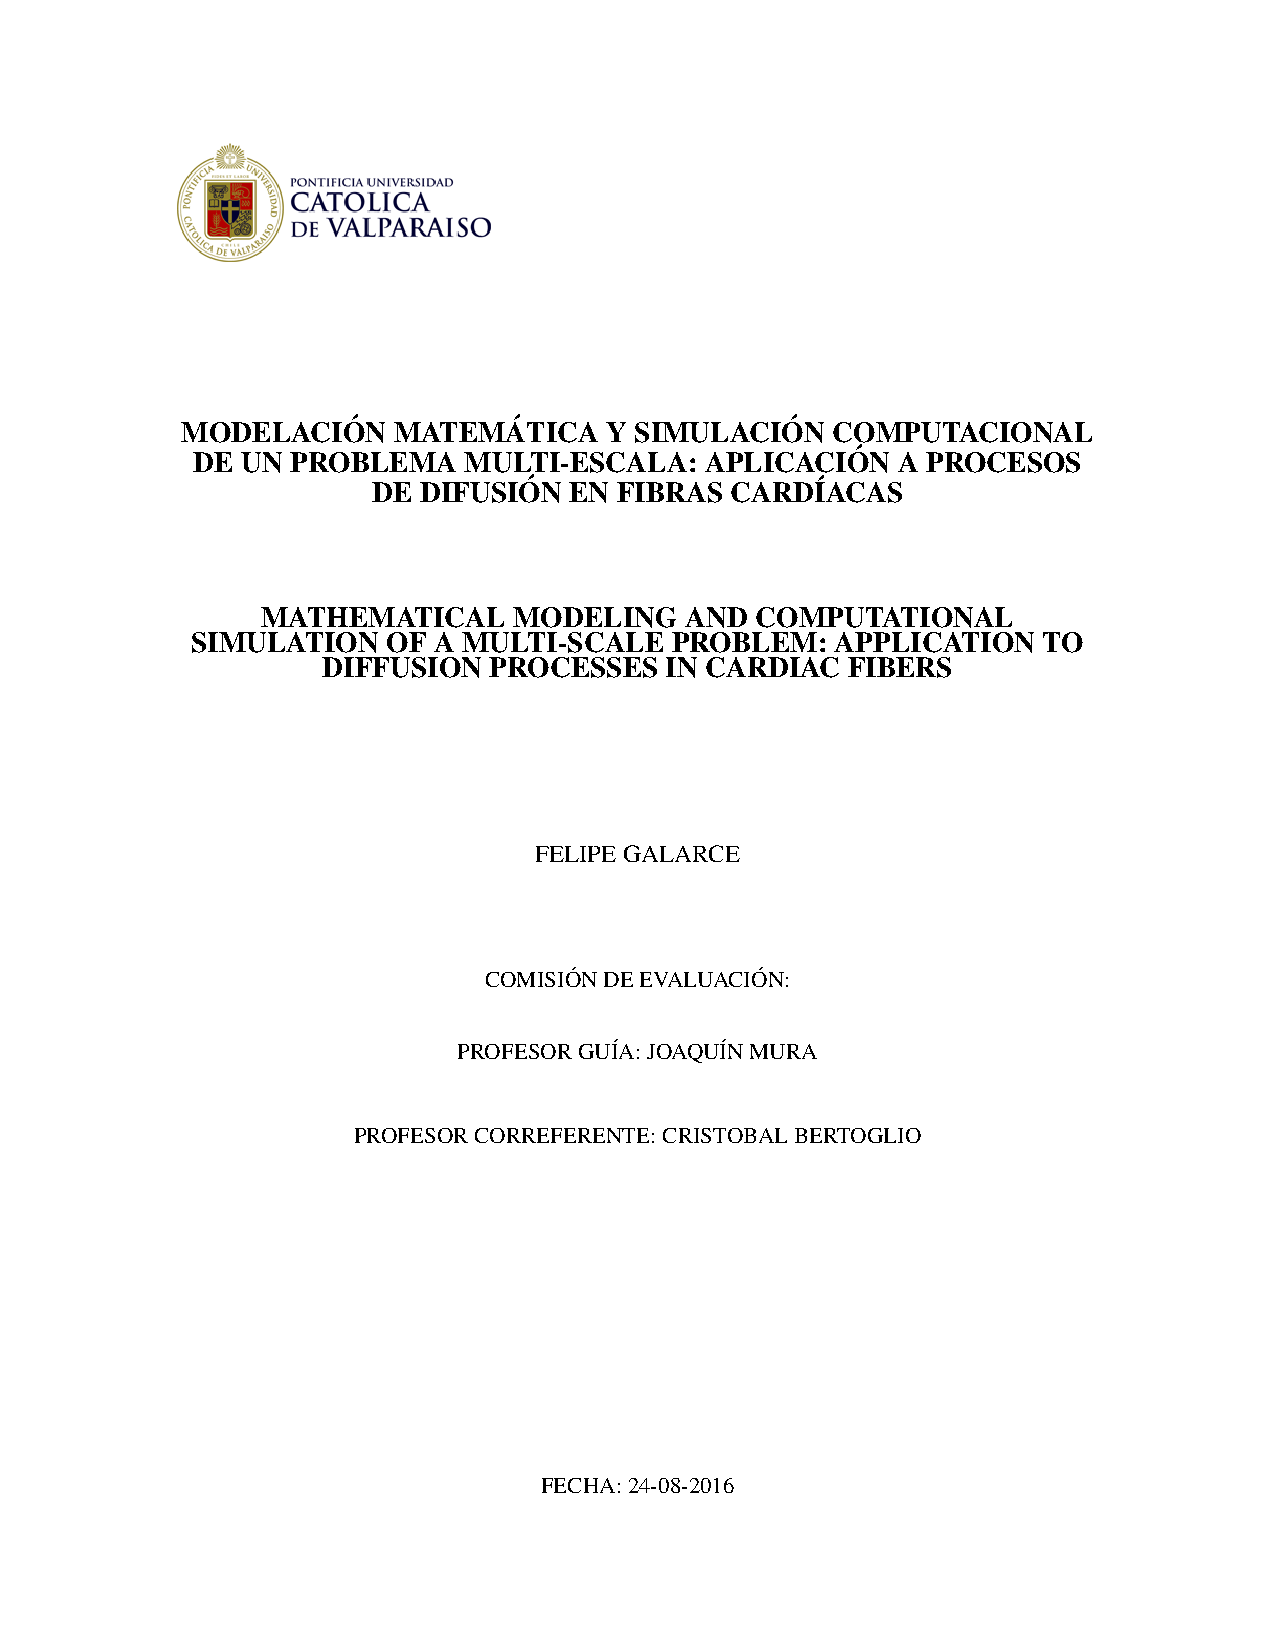
\includepdf[pages=1]{build/PORTADA.pdf}

%====================================

% Re-enable page-numbering
\pagenumbering{arabic}
% Define vertical space for the rest of the document (equivalente a interlineado sencillo en Microsoft Word)
%\spacing{1}
% Reset page counter in order to not consider the titlepage
%\setcounter{page}{1}
% Set font size
%\fontsize{11}{12}\selectfont

\tableofcontents
\newpage

% Consider abstract into table of contents
\addcontentsline{toc}{section}{RESUMEN} 
\addcontentsline{toc}{section}{ABSTRACT} 


\includepdf[pages=2]{./build/Abstract.pdf}

\newpage

\newpage

\section{1. INTRODUCTION}

\newpage

\section{2. AIMS}

\newpage
\section{SOME BASIS ON ANATOMY AND ELECTROPHYSIOLOGY} \label{Some_Basis_on_Anatomy_and_Electrophysiology}

The heart is a double pump consisting of four chambers, two atria in the upper part, separated by the inter-atrial septum and two ventricles in the lower part, separated by the inter-ventricular septum. See (\ref{corazon}) for a schematic and \cite{electrofis} for more details. The hearth function is achieved by a complex interaction between the electrical and mechanical activity.

\begin{figure}[H] % esquema corazón
\centering
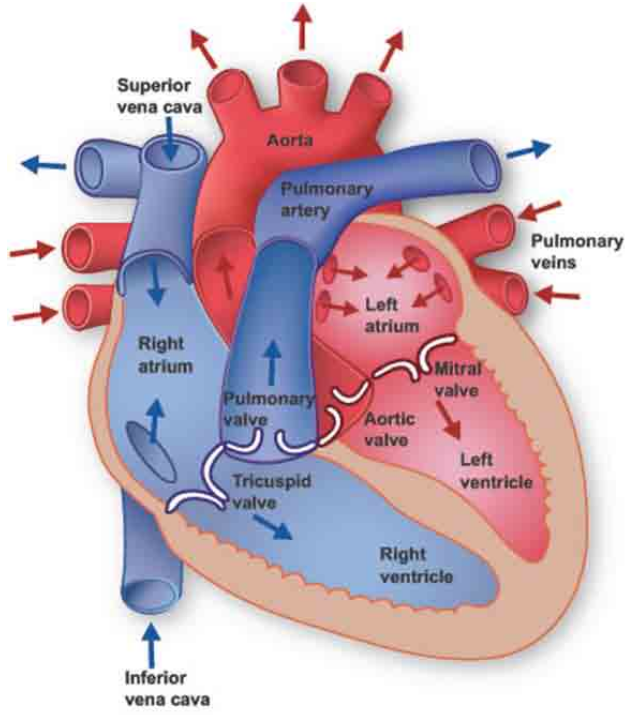
\includegraphics[height = 7 cm]{fig/fundamentals-corazon}
\caption{schematic diagram of the heart anatomy. From \cite{texas_inst} } \label{corazon}
\end{figure}

The electric wave genesis responsible of the contraction of cardiac muscle cells occurs due to an autonomous depolarization in the sinoatrial node (SAN), located in the upper part of right atria. Then, the propagation is achieved cause this depolarization changes the membrane potential of surrounding cardiac cells (due,  actually, to a membrane ionic flow).

Obviously, the potential travels first in the right atria, then into the left one. Later the atrio-ventricular node (AVN) is reached, which conveniently has a high electric resistivity, in order to generate a control delay in the propagation, preventing and early ventricular stimulation. Finally, the Purkinge network enable a fast potential propagation to ventricles. The previous can be appreciated in the figure (\ref{corazon_conduccion})

\begin{figure}[H] % esquema conducción de corriente en el corazón
\centering
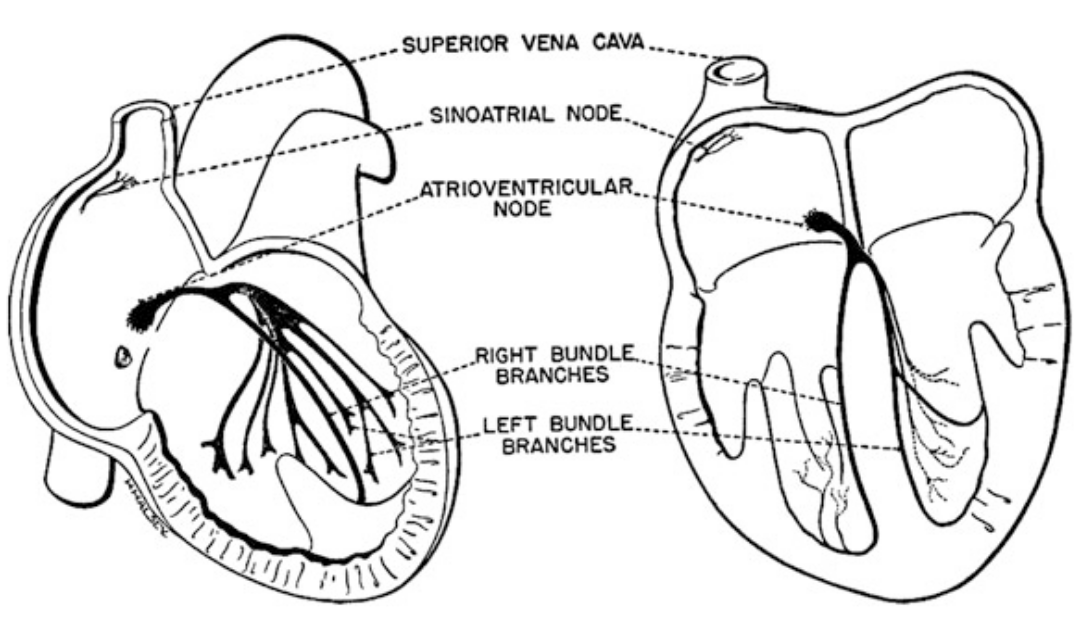
\includegraphics[scale=.4]{fig/fundamentals-sistema_de_conduccion}
\caption{schematic diagram of the heart conduction system. From \cite{electrofis}} \label{corazon_conduccion}
\end{figure}

\subsection{Cardiac Tissue Organization} \label{Cardiac_Tissue_Organization}

The contract/relax macroscopic behaviour of the heart is achieved due to the collective myocites activity. This cells works together joint by \textsl{gap junctions} that allows a quick electrical propagation. Every of this myocites has a an internal protein arrays called myofibrils, as can be seen in fig. (\ref{fig:myocite}), which enables most part of the elastic properties of the cardiac tissue.

\begin{figure}[H]
\centering
\subfigure[schematic view of a myocite.]{
    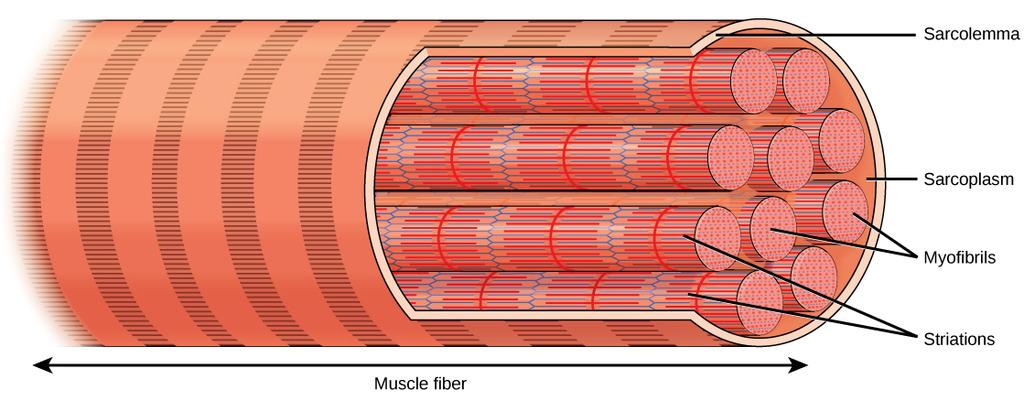
\includegraphics[scale=.35]{fig/fundamentals-myocites}
    \label{fig:myocite}
}
\subfigure[gap junctions. ]{
    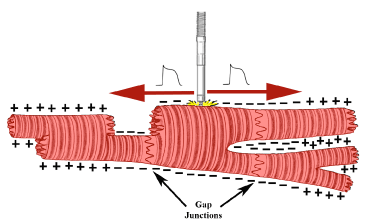
\includegraphics[scale=.6]{fig/fundamentals-gap_junctions} 
    \label{fig:gap_junctions}
}
\caption{the cardiac muscle cells and its sarcoplasma electrical bypass.} 
\end{figure}

Also, in the cardiac tissue exist another type of cells called \textsl{fibroblasts}, who are responsible of synthesize the extracellular matrix (ECM), an extensive and highly organized network of fibrous proteins, elastic and collagen (the main structural protein of the extra-cellular space in the human and other animals connective tissue). Specifically, the fraction of this last protein can be used as a measure between a healthy and a damaged by fibrosis heart. 

Now, the myocites and the ECM are arranged together in a complex three-dimensional spatial organization, with a fiber and laminar structure, like in figure (\ref{orientacionmiocitos}). This organization, as can be expected, affects the diffusion properties of the tissue, which is highly anisotropic. This last usually is represented by a second-rank tensor, that can be written as a $3 \times 3$ matrix. The three orthogonal eigenvector of this tensor can be related directly to cardiac structure. In fact, the primary eigenvector (i.e. the eigenvector with the largest eigenvalue) will be along the fiber long axis, the secondary eigenvector will lie orthogonal to fiber long axis, in the myolaminar plane, while the minor eigenvector, orthogonal to the other two, will be normal to the myolaminar plane.

\begin{figure}[H]
\centering
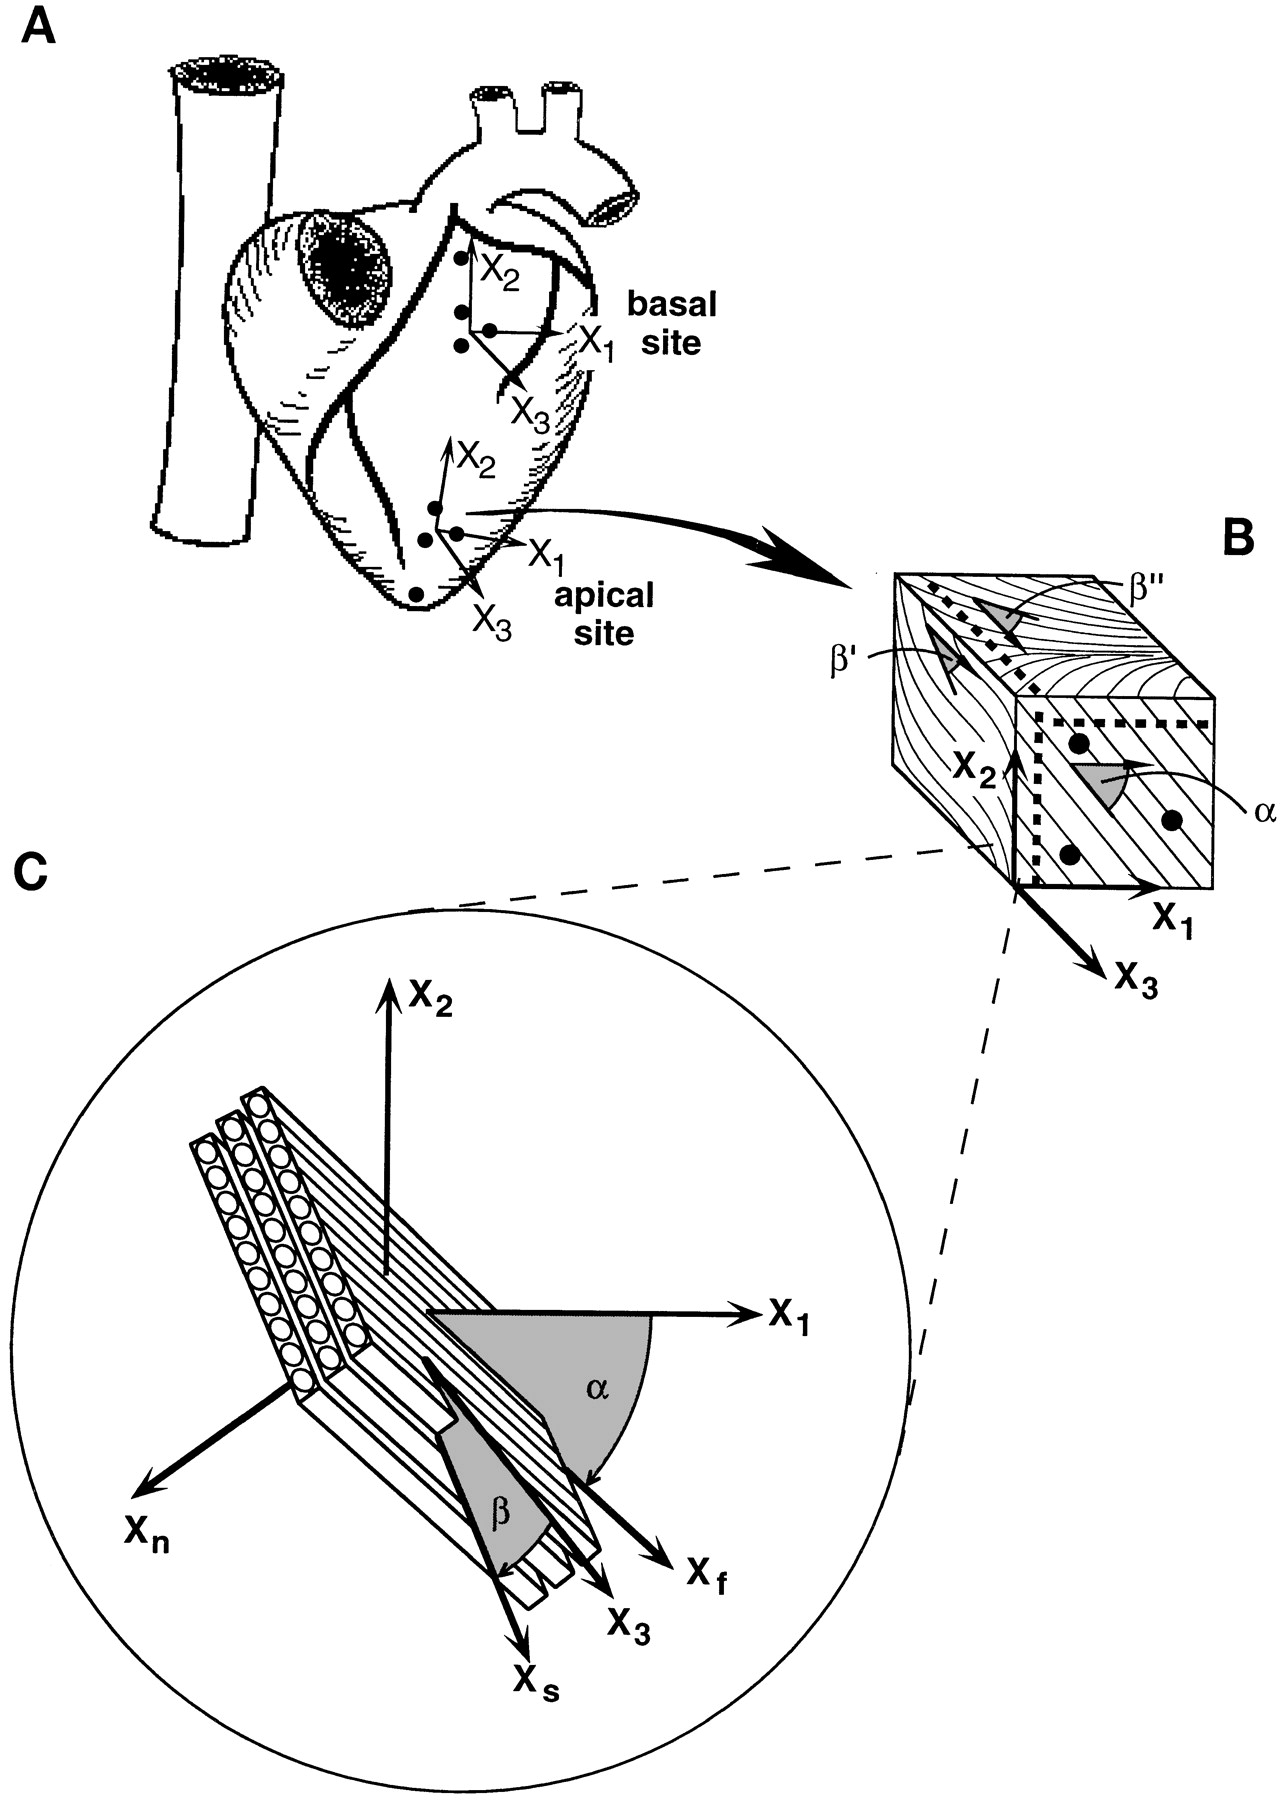
\includegraphics[scale=.14]{fig/fundamentals-direccionmiocitos}
\caption{heart fiber orientation. From: \cite{shearstrain-fiberorientation}} \label{orientacionmiocitos}
\end{figure}

\subsection{Action Potential} \label{Action_Potential}

As established above, cardiac cells are excitable cells, some autonomously and some after a proper electrical stimulus. The excitation of a cardiac cell causes a rapid variation of its potential difference across the cell membrane, the so-called \textsl{transmembrane potential}. There exist a minimum value of potential difference stimulus below the cell will react, a threshold, that if is reach, the cell membrane depolarizes and the trans-membrane potential change from a resting negative value to a slightly positive one. This complete event is called an \textsl{action potential}, and phases can be identified, according to the activation of different membrane ionic channels. One action potential cycle can be seen in figure \ref{action-potential}. 

\begin{figure}[H]
\centering
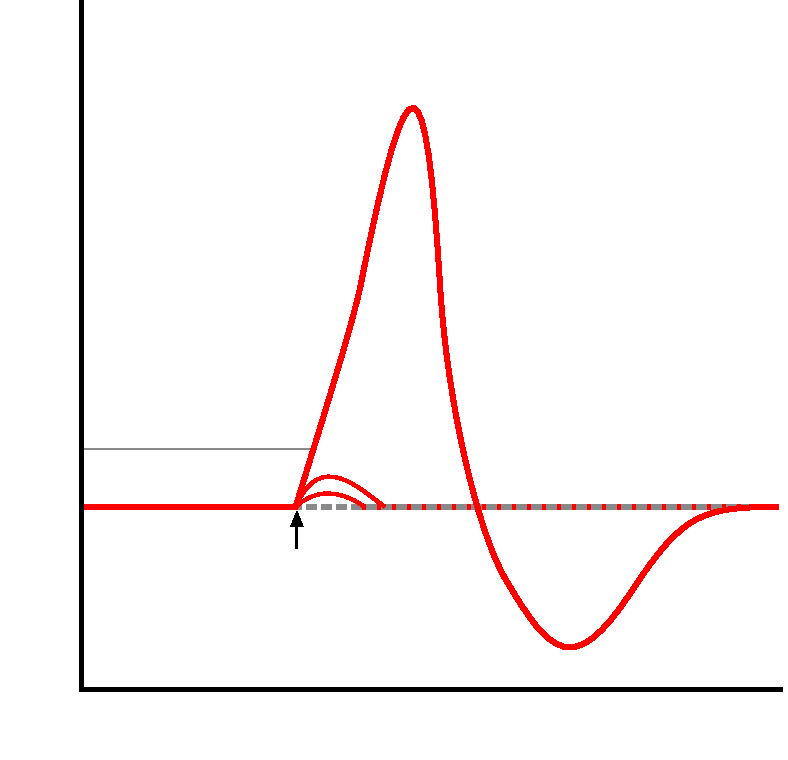
\includegraphics[height = 7 cm]{fig/fundamentals-action_potential}
\caption{squematic plot of a cardiac action potential with its phases. Fuente: \cite{action-potential-figure}} \label{action-potential}
\end{figure}

The extracellular potential due to the propagation of action potentials can be registered in a electrocardiogram (ECG), which can eventually lead us to diagnose some diseases as consequence of the fibrosis, as the sinus bradycardia and tachycardia, arrhythmias, paroxysmal atrial tachycardia, ettc.

\subsection{Fibrosis} \label{Fibrosis}

As we say in the introduction, the cardiac fibrosis is the excess of fibrous connective tissue, like collagen, as consequence of an auto-regenerative process done by the fibroblasts. 

Different patterns of fibrosis has been observed, considering the percentage of extra connective tissue (density of fibrosis) and the dispersion of fibrotic areas in the tissue, i.e., the spatial distribution of the fibrosis. Furthermore, according to the last parameters, can be defined  different types of fibrosis (see \cite{Kawara2001Circ}), as \textsl{stringy}, \textsl{diffuse} and \textsl{patchy}. The stringy pattern is characterized by homogeneously distributed fibrosis with long and single strands, in the patchy pattern apears long and compact groups of strands, while in the diffuse pattern appears more or less diffusely distributed fibrosis with short strands. In figures \ref{fig:stringy}, \ref{fig:patchy} and \ref{fig:diffuse} can be observed sections of a heart with the different patterns of collagen accumulation established above. 

\begin{figure}[H]
\centering
\subfigure[stringy Fibrosis.]{
    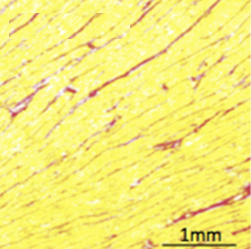
\includegraphics[width = 5 cm]{fig/fundamentals-fib-stringy}
    \label{fig:stringy}
}
\subfigure[patchy Fibrosis. ]{
    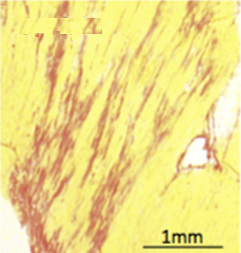
\includegraphics[width = 5 cm]{fig/fundamentals-fib-patchy} 
    \label{fig:patchy}
}
\subfigure[diffuse. ]{
    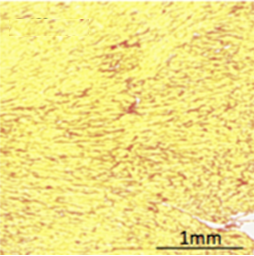
\includegraphics[width = 5 cm]{fig/fundamentals-fib-diffuse} 
    \label{fig:diffuse}
}
\caption{different types of fibrosis.}
\end{figure}

The remarkable thing is that some studies \cite{Comtois2011IEEE} suggest that when a density threshold is reach, only this spatial distribution of connective tissue affects in the propagation velocity of the potential. In a research by Kawara \cite{Kawara2001Circ}, the mean increase of the delay in the propagation (MID) was measured for failed hearts with different density of fibrosis. A result of this study can be seen in figure \ref{fig:midvsdensity}.

\begin{figure}[H]
	\centering
	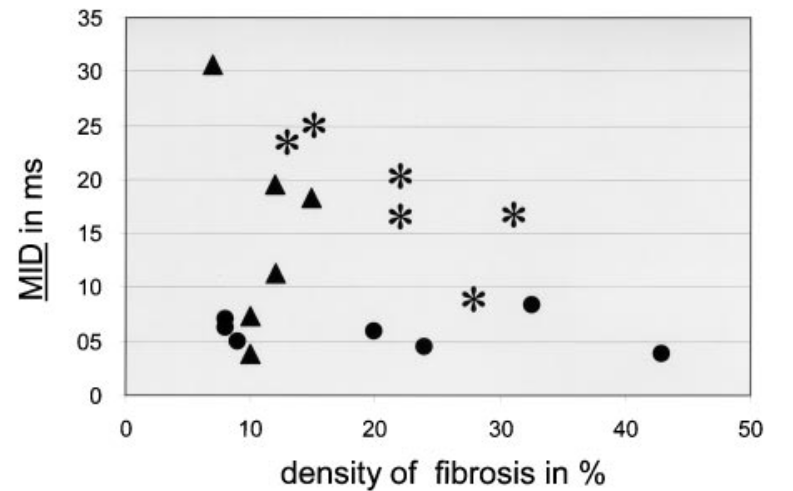
\includegraphics[width= 8 cm]{fig/fundamentals-fib-midvsdensity}
	\caption{scatterplot of density of fibrosis and MID for different types of fibrosis (patchy, $*$; stringy, $\blacktriangle$; or diffuse, $\bullet$) . From \cite{Kawara2001Circ}}. \label{fig:midvsdensity}
\end{figure}

Note that high values of MID are usually associated with patchy or stringy fibrosis. In areas with diffuse fibrosis, low values of MID are found, even at high densities of fibrosis.

The main objective of this document is the study of the interaction between the density and dispersion of this pathology and the propagation velocity of the electric potential. So, the next sections will be focused on mathematical modelling the potential diffusion in the cardiac tissue, considering the laminar architecture described below, as well as the individual cell behaviour due to the action potential.
\end{document}
